%
% Modified by Megan Patnott
% Last Change: Jan 18, 2013
%
%%%%%%%%%%%%%%%%%%%%%%%%%%%%%%%%%%%%%%%%%%%%%%%%%%%%%%%%%%%%%%%%%%%%%%%%
%
% Modified by Sameer Vijay
% Last Change: Tue Jul 26 2005 13:00 CEST
%
%%%%%%%%%%%%%%%%%%%%%%%%%%%%%%%%%%%%%%%%%%%%%%%%%%%%%%%%%%%%%%%%%%%%%%%%
%
% Sample Notre Dame Thesis/Dissertation
% Using Donald Peterson's ndthesis classfile
%
% Written by Jeff Squyres and Don Peterson
%
% Provided by the Information Technology Committee of
%   the Graduate Student Union
%   http://www.gsu.nd.edu/
%
% Nothing in this document is serious except the format.  :-)
%
% If you have any suggestions, comments, questions, please send e-mail
% to: ndthesis@gsu.nd.edu
%
%%%%%%%%%%%%%%%%%%%%%%%%%%%%%%%%%%%%%%%%%%%%%%%%%%%%%%%%%%%%%%%%%%%%%%%%


%
% Chapter 4
%


\chapter{Measured lifetimes}
\label{chap: lifetime}

This chapter presents the details of the analysis used for the determination of the lifetime of the 6.79 MeV state, the 5.18 MeV state, and the 6.17 MeV state in $^{15}$O. These data resulted from a nine-day long experiment at the university of Notre Dame Nuclear Science Laboratory in August 2019. This measurement used protons from the 5U Sta. Ana accelerator for the $^{14}$N(p,$\gamma$)$^{15}$O reaction at beam energies ranging from 1 MeV to 1.6 MeV. Further description of this experimental setup, targets, and methodology can be found in Chapter \ref{chap: experiment}.	

\section{Determining a nuclear lifetime}
\label{sec: lifetime determination}

For this analysis, a new DSAM program was written to simulate the expected Doppler shift and lineshape. This approach, as will be outlined shortly, follows the Monte Carlo (MC) technique for simulating physical phenomena with the sampling of random numbers. A full reproduction of the code is provided for reference in Appendix \ref{appendix: codes}. 

The MC technique is simple enough in idea and a powerful tool across the fields of physics and mathematics: to numerically estimate phenomena by studying their effects with reasonably sampled, random numbers. In other words, the aim is to build a probability distribution that is proportional to some function, $P(x)$, which spans the interval $[x_{min}, x_{max}]$, using random numbers in the range [0,1]. To start, take the integral of the function over some subset of its total range,

\begin{equation}
I(x) = \int_{x_{min}}^{x} P(x') dx',
\label{eqn: mcStart}
\end{equation}

\noindent where $x_{min} \leq x \leq x_{max}$. Normalizing this integral to the integral over the complete range,

\begin{equation}
I_{norm}(x) = \dfrac{I(x)}{I(x_{max})} = \dfrac{\int_{x_{min}}^{x} P(x') dx'}{\int_{x_{min}}^{x_{max}} P(x') dx'},
\end{equation}

\noindent creates the desired relationship, since the integrated probability is itself a random variable and the normalization guarantees its range is confined to [0, 1]. This is shown when evaluating $I_{norm}$ at the extremes of its domain,

\begin{equation}
I_{norm} (x_{min}) = \dfrac{\int_{x_{min}}^{x_{min}} P(x') dx'}{\int_{x_{min}}^{x_{max}} P(x') dx'} = 0
\end{equation}

\noindent and

\begin{equation}
I_{norm} (x_{max}) = \dfrac{\int_{x_{min}}^{x_{max}} P(x') dx'}{\int_{x_{min}}^{x_{max}} P(x') dx'} = 1.
\end{equation}

\noindent Finally, then, to utilize this relationship in the MC technique, $I_{norm}$ is evaluated for a specific function and ultimately inverted to produce a response in the original function, $P(x)$, as a function of a randomly generated number in the range of [0, 1].

Specifically, the case of interest in this work involves the modeling of exponential decay,

\begin{equation}
P(x) = e^{-\lambda x},
\end{equation}

\noindent where $\lambda$ is the width and inversely proportional to the lifetime, $\lambda = 1/ \tau$. In this context, the domain of input variable, $x$, is [0, $\infty$], as the decay can occur at any time. Utilizing this in the formulation starting with Equation \ref{eqn: mcStart},

\begin{equation}
I(x) = \int_{0}^{x} e^{-\lambda x'} dx' = \frac{1}{\lambda} (1 - e^{-\lambda x}),
\end{equation}

\begin{equation}
I(x_{min}) = I(0) = 0,
\end{equation}

\begin{equation}
I(x_{max}) = I(\infty) = 1/\lambda,
\end{equation}

\noindent and, ultimately, 

\begin{equation}
I_{norm}(x) = \frac{\lambda^{-1}(1 - e^{-\lambda x})}{\lambda^{-1}} = (1 - e^{-\lambda x}).
\label{eqn: exponentialGenerator}
\end{equation}

\noindent An example of this approach is plotted for reference in Fig.\ \ref{fig: expoGen}. This plots Equation \ref{eqn: exponentialGenerator} for the arbitrary choice of $\lambda$=50 to demonstrate the operational principles. The range of this function's response is limited to [0, 1], as it approaches 1 asymptotically. While the input variable, decay time, is only plotted to 0.1 in this figure, the behavior does not change at higher values and was only chosen to highlight this method. Now, a random number, $r$, can be generated on the range [0, 1], i.e.\ within the range of $I_{norm}(x)$, and this curve can be used to look up and identify a value for the specific decay time, $x$. 



\begin{figure}
\thisfloatpagestyle{plain}
\centering
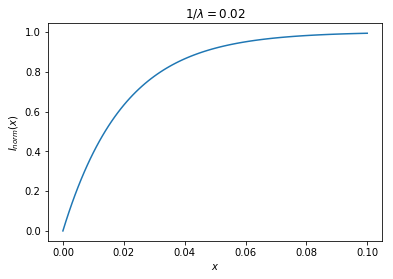
\includegraphics[width=0.85\linewidth]{figures/expoDecayGenerator.png}
\caption{An example of the Monte Carlo method for constructing a relationship between a function and the random number generator. This plots the $I_{norm}(x)$ of Equation \ref{eqn: exponentialGenerator} for an arbitrary choice of $\lambda = 50$ to demonstrate the technique. The range of the response of this function is limited to [0, 1] asymptotically, while the input variable of decay time is unrestricted. }
\label{fig: expoGen}
\end{figure}


However, this can be more instructive to invert the function and create a relationship to output a decay time for a randomly generated $r$ and a given width and lifetime, $\lambda$ and $\tau$, respectively.  This is done as,

\begin{equation}
r = 1 - e^{-\lambda x} \Rightarrow e^{\lambda x} = \dfrac{1}{1-r} \Rightarrow x = \dfrac{1}{\lambda} \ln \left( \frac{1}{1-r} \right).
\label{eqn: rand}
\end{equation}

\noindent The above relationship is then used to simulate a decaying nucleus. By selecting a random number within [0, 1] one can determine the corresponding decay time of a nucleus with a given lifetime from Equation \ref{eqn: rand}. For a large amount of randomly generated numbers, the general behavior of the initial function, exponential decay in this case, can be simulated and studied. An example of this is shown in Fig.\ \ref{fig: simExample} for 100,000 such events. The total behavior can be stored and compared with the original decay law. To do this, however, the simulated histogram must be normalized to match the properties of the original function, $P(x)$.  Namely, the survival cannot be greater than 1, and, indeed, $P(0) = 1$. Therefore, by normalizing the whole histogram to the value of the first histogram bin, the simulated decay curve can be compared to the function from which it was generated. As Fig.\ \ref{fig: simCompare} demonstrates, this is a effective and faithful method of simulating these natural phenomena. 


\begin{figure}
\centering
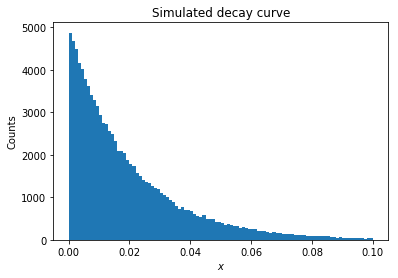
\includegraphics[width=0.85\linewidth]{figures/simExample.png}
\caption{An example of the Monte Carlo method for a simulated decay curve. For 100,000 simulated nuclear decays with a $\lambda$=50, the MC method generates the given histogram of decay times.  }
\label{fig: simExample}
\end{figure}


\begin{figure}
\thisfloatpagestyle{plain}
\centering
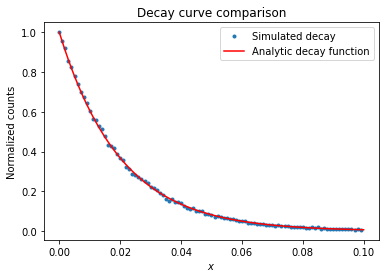
\includegraphics[width=0.85\linewidth]{figures/simCompareExample.png}
\caption{An example of the Monte Carlo method for a simulated decay curve. For 100,000 simulated nuclear decays with a $\lambda$=50, the MC method generates the given histogram of decay times.  }
\label{fig: simCompare}
\end{figure}


It is upon these principles and this derived formulation that the experimentally measured nuclear lifetimes were extracted. 

SRIM \cite{Ziegler2010}


\section{Systematic errors}
\label{sec: systematicErrors}

\section{Lifetime of the 5.18 MeV state in $^{15}$O}
\label{sec: lifetime518}


\section{Lifetime of the 6.17 MeV state in $^{15}$O}
\label{sec: lifetime617}


\section{Lifetime of the 6.79 MeV state in $^{15}$O}
\label{sec: lifetime679}

% % uncomment the following lines,
% if using chapter-wise bibliography
%
% \bibliographystyle{ndnatbib}
% \bibliography{example}
